\documentclass[12pt]{article}
\usepackage[lmargin=2cm,rmargin=2cm,bmargin=3cm,tmargin=2cm]{geometry}
\usepackage{amsmath,amssymb} 
\usepackage{graphicx} 
\usepackage{float}
\usepackage{multicol} 
\usepackage{hyperref} 
\hypersetup{pdfinfo={
Title={Connect: A Distributed Message Board}, Author={Irtiza Ahmed Akhter,
Zainab Ghadiyal}, }}

\title{Connect: A Distributed Message Board} 
\author{Irtiza Ahmed Akhter\\
\texttt{irtiza@cs.wisc.edu} \and Zainab Ghadiyali\\ \texttt{zainab@cs.wisc.edu}}

\begin{document} 
\maketitle

\section{Abstract} 

Distributed Systems are widely popular and increasingly
important given the yearly increase in number of Internet users and scalable
systems. In this paper, we describe the design, implementation and analysis of
Connect, a distributed system built on top of Amazon's EC2 service. Web stress
testing shows that latency is directly proportional to the number of users
on-line. Query completion time is linear proportional to number of queries
running in parallel. \emph{MySQL} replication, although tedious to implement, can
provide an effective open-source based solution to ensuring data replication
across servers. Effective load balancing and an eventually consistent replication model 
is implemented and verified.

\section{Introduction} 
\label{Introduction}

The increasing ubiquity of distributed systems utilized for communication has
paved way for an increasing number of advances. Deploying a communication tool
over a distributed system can be done in several ways. Internet Relay Chat (IRC)
is one of the oldest communication tools found on the Internet. The backbone
structure is a spanning tree of servers and users connect to one of these
servers. The message then trickles down to all servers across the spanning tree.
The protocol is simple and widely studied. Another type of tool is web based
with each chat application differing in interface and functionality. AOL Instant
Messenger, Facebook Messenger and Google Chat are some examples dominating this
space.
 
\subsection{IRC} 

Internet Relay Chat(IRC\cite{IRC}) was a rather widely used
communication tool. Each IRC network comprises of a spanning tree structure of
servers who typically listen on port 6667. A user identifies himself within the
IRC-network through a designation user name. The user name is hence unique within
a particular network.  IRC networks comprise of several channels which form
meeting and discussion avenues. Since channels are so critical to IRC
functioning, it is imperative that these channels be unique and consistent
throughout the network. An IRC operator works as an administrator to override actions of
remove users from network.  

\subsection{Web-chat} 
A web communication tool uses a browser as a user interface and HTTP as underlying 
application protocol. Typically, a web chat service has a login system to 
authenticate users and a session id to maintain consistency and ensure that each 
user gets the chat message that are sent by other user(s).  

\subsection{Design} 
In our communication tool we use the TCP protocol for communication between the server 
and client while communication between the client and location server is via HTTP and TCP. 
TCP is a connection oriented reliable protocol and states related to each TCP 
connection need to be maintained at both client and server side. UDP could be used 
for transfer of messages, however we choose TCP over UDP due to TCP's reliability and the fact
that packet loss may occur.  The application is to be implemented using a
client server architecture as follows: 

\begin{enumerate} 
\item Clients connect to a server after signing up via an internal log-in system or external log-in
system (Facebook Connect) 
\item Server is responsible for broadcasting the log-in messages 
\item Since the chat server has the key role of transmitting and storing messages, it is 
important to automate the chat server as much as possible in order to improve operational performance.  
\item The client must be able to use the chat service irrespective of changes to the chat server and internal application
network.  
\item The clients must be able to connect to the chat server irrespective of firewalls.  
\item The client must have easy access to the chat
application through all major browsers 
\end{enumerate} 

\section {Design and Implementation of Front-End Features} 
Connect provides a simple, easy to use interface to minimize delays due to poor product design. 
The landing page comprises of a log-in section, allowing registered users to access Connect. In
order to learn to work with data integrated from another distributed
system, as well as to provide a quick and convenient way for our users to access
Connect, we integrate a Facebook Connect button. This allows users to register
and log-in to Connect via their Facebook account. Unregistered users unwilling
to utilize Facebook connect may use a simple registration form to create an
account.  After log-in has been successfully authenticated, users are transfered
to the message board. This message board has also been designed keeping ease of
use in mind. The page is chiefly divided into three sections: 
\begin{enumerate}
\item Top right: A list of logged in users.  
\item Top left: A list of messages
\item Bottom : A text area to input messages 
\end{enumerate} 
Additionally, we also ensure to implement the following features in the front end application: 
\begin{enumerate}
\item The application is very lightweight, that is it does not consume too much client bandwidth
\item It can be used by almost all the browsers available to this date
\item In the website through out all the pages, we have implemented \emph{Ajax} based sanity checks to validate different user inputs to different \emph{HTML} forms before submitting to the server side \emph{PHP} script (e.g. notifying the user in case of an input email address having improper format).
\item Users can see which other users are currently connected
\item Messages are never lost, that is a user can log in and see all the messages posted by 
other users during the period s/he was not connected
\end{enumerate}

\section {Design and Implementation Of Distributed Back-End} 
We aim to design the back-end to provide the following features:
\begin{enumerate}
\item Load balancing
\item Data replication
\item High availability
\item Eventually consistent replicas
\item Scalability/replication of service
\item Fault tolerance
\item Automated recovery. 
\end{enumerate}
In this section we will cover each of these features and corresponding implementation 
one by one. In general, we wanted to automate as many features as possible in order to 
minimize human intervention and to provide higher degree of 
transparency to the end-users. Before going into the implementation details, we will first
present a brief overview of the tools and techniques we have used for that will
be helpful for the reader to understand the limitations of the services provided
by these tools and our implementation specific corresponding solutions.

\subsection{Tools} 

\begin{figure}[H] 
\centering
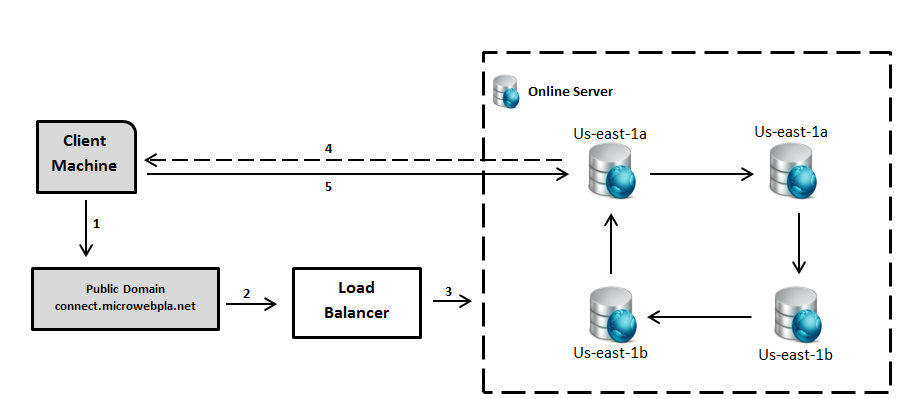
\includegraphics[scale=0.60]{Images/figure1.PNG} 
\caption{\textbf{Work-flow: }We
have set up a public domain to make the service available to the Internet users.
A client request first goes to \url{connect.microwebpla.net}(1), microwebpla.net points
to the load balancer (2), the load balancer picks a suitable target server from
the cluster and forwards the original request (3), the selected server gets back
to the client with a reply and establishes a virtual communication channel (4),
until the channel is closed, from this point client directly communicates with
the selected server in step (3).} 
\label{fig:workflow} 
\end{figure} 

Our distributed message board application was built using several tools. Firstly we
used \emph{Amazon's Elastic Cloud Computing (EC2)} \cite{ec2} instances to
accommodate the \emph{web servers} and the \emph{database} servers. We spawned
four  \emph{t1-micro EC2} \cite{t1micro} instances in two separate geographical
zones (Us-east-1a , Us-east-1b) for this purpose. Four instances were utilized
since it allowed us to better test and implement system in the time frame
provided without compromising on any distributed systems feature implemented and
analyzed. Two geographical regions helped better study performance and load
balancing due to geographical differences in where servers were placed. All the
\emph{EC2} instances are of type \emph{t1-micro} and have identical configuration with.
\emph{Ubuntu 11.14} (32 bit) as the operating environment. Next
we installed \emph{Apache Web Server} \cite{apache} to host the web pages and
\emph{MySQL} \cite{mysql} as the database to accommodate our simple data
structure. We used a fifth \emph{EC2} instance as a the \emph{Load Balancer}. In
order to make the service accessible from a domain name, we have setup a public
domain (\emph{connect.microwebpla.net}) whose DNS records point to the load balancer. 
Namely, we have added a CNAME \cite{cname} record for the sub-domain
\emph{connect.microwebpla.net} to make it an alias of the load balancer. The
domain and its DNS records are managed by \emph{Name.com}. We used \emph{PHP},
basic \emph{HTML} and \emph{JQuery} \cite{jquery} to write the front end
application, \emph{MySQL} and \emph{Shell Script} on the back end to implement
different features of distributed system such as - load balancing, replication,
fault tolerance, etc. And finally, the entire setup involved writing a number of
custom configuration scripts for \emph{Apache}, \emph{MySQL} and \emph{EC2}
instances. In  \textbf{Figure}~\ref{fig:workflow} we have laid out the different
components of the entire system and presented the work-flow of serving a client
request from a high level. In the following sections we will present several
distributed aspects of our design.

\subsection{Replication and Consistent Update Propagation} 
The goal of replication may be considered two-fold in nature. Firstly, services are
replicated across all back-end nodes, thus enabling any back-end node to serve
any client request. Secondly, stored data is replicated in as many instances as
possible for higher availability. The first one can be interpreted as serving the web pages and accepting \emph{MySQL} queries, which turned out be very straight forward. We simply replicated the web server with
the web pages and the \emph{MySQL} tables in all the instances. This way each
\emph{EC2} instance can serve the same web application to the end-users
transparently. The latter however turned out to be tricky. Every web server is
coupled with a \emph{MySQL} instance, however it is not strictly necessary to
forward a specific database operation from a web server to the \emph{MySQL}
instance it is coupled with, we will elaborate more on this in \textbf{section}
\emph{\ref{lb.a.t}}. The second goal of replication is strictly tied to data
availability and consistency. We wanted to design such a system, where data will
be replicated almost instantly in all the database instances regardless of the
location of the server that first accepts and processes the request, and thus
providing \emph{eventual consistency}. For that, at one point we decided to write code
from the scratch to propagate the updates from one instance to the other. Then
again, keeping in mind the fact that we did not want to re-invent the wheel, we
researched a little bit more and found out that the latest \emph{MySQL}
installation offers a model for replication \cite{mysql-replication}(\textbf{Figure}~\ref{fig:mysqlreplication}).  
\begin{figure}[H] 
\centering
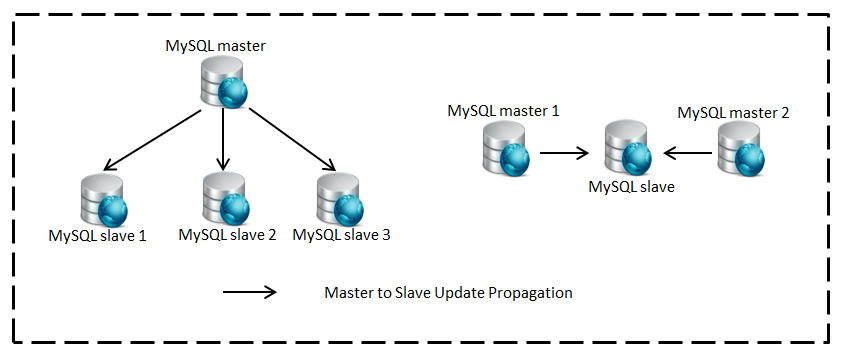
\includegraphics[scale=0.80]{Images/figure6.PNG} 
\caption{\textbf{MySQL Replication and Limitation:} 
\emph{Left: }Native MySQL Replication. Single master, multiple slaves, unidirectional 
write propagation model.  
\emph{Right:}
Our requirement is multi master, multi slave and bi-directional model to support
absolute replication, higher availability of service and strong consistency. To
this date, MySQL does not have any support for this model.}
\label{fig:mysqlreplication} 
\end{figure} 

\emph Our model of replication is adopted from {MySQL} whose design goals and use cases are different from ours. 
The use case of this model is to backup existing database(s) to one or more shadow servers
from a single master database. For this reason, the \emph{MySQL's} replication
model allows one \emph{master} replica to propagate updates to one (or more)
\emph{slave} replicas, so that in case of a \emph{master} failure the
\emph{slave} can take over without loosing any data
\textbf{Figure}~\ref{fig:mysqlreplication} (left). Note that,  (1) this model
only allows a \emph{master} $\rightarrow$ \emph{slave} update propagation, in
other words propagation is unidirectional, (2) a single \emph{master} can have
multiple \emph{slaves}, but a single \emph{slave} cannot receive updates from
multiple \emph{masters}, (3) this model imposes the concept of \emph{master} and
\emph{slave} and thus making the master a single point of failure and isolation
of service and (4) the process of promoting the \emph{slave} replica to become a
\emph{master} during a failure is not automated. Because of these limitations,
this model is not adequate for our design goals. The first three limitations
directly affect our design goals for replication, availability and consistency
and the last one affects fault tolerance and recovery (we discuss this in
\textbf{Section} \ref{fault})\\
Next we focused on how to leverage this existing replication model to ease our implementation at the same time not compromising any of the design goals. The intuitive  solution we came up with can be deemed
as a \emph{ring topology}, where each node in the ring is a \emph{MySQL}
instance acting both as \emph{master} and \emph{slave} (thus eliminating the
distinction between these two roles). As shown in \textbf{Figure}~\ref{fig:connectreplication}, 
update always propagates from \emph{master} to \emph{slave} in one direction. 
This update propagation can be seen as influenced by \emph{Bayou's Anti Entropy} protocol, 
where each server talks to some other server and transfer the latest updates received by the first
and unknown to the second (maintaining prefix property to have incremental write
propagation). However to achieve this we had to experiment with configurations,
as in the ring, each instance is a \emph{master} of its successor and
\emph{slave} of its predecessor at the same time which is not supported by
\emph{MySQL} natively. Again this concept is highly related to our availability
goal we mentioned before. Each instance should be able receive update as a
\emph{master}, log the update and propagate to its appropriate successor. All
instances will have to be synchronized with their corresponding \emph{master}
and \emph{slave} neighbors in terms of log position.  
\begin{figure}[H]
\centering 
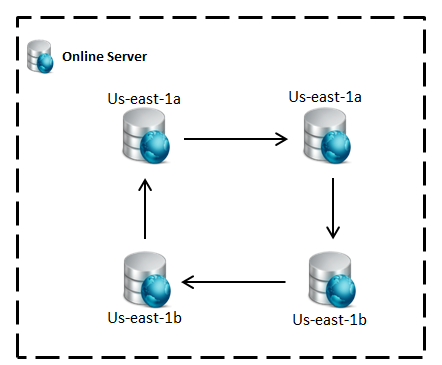
\includegraphics[scale=0.8]{Images/figure2.PNG} 
\caption{\textbf{Data Replication to Provide Eventual Consistency: }All the servers are connected to
each other forming a daisy chain. Data flows unidirectionally from one
\emph{master} to its single \emph{slave}. } 
\label{fig:connectreplication}
\end{figure} To keep the description succinct we are skipping the low level
technical details. But the above design indeed gave us a very robust replication
model. However this introduced new challenges to handle failure situation and
inconsistent log position. We will talk about that in the next section. It is
worth pointing out that we leveraged the original \emph{MySQL} replication model
without any violation. To be precise, in our model updates still flow
unidirectionally from a single \emph{master} to \emph{slave}.
\subsection{Automated Failure Detection And Self Healing}
\label{fault}
\begin{figure}[H] \centering 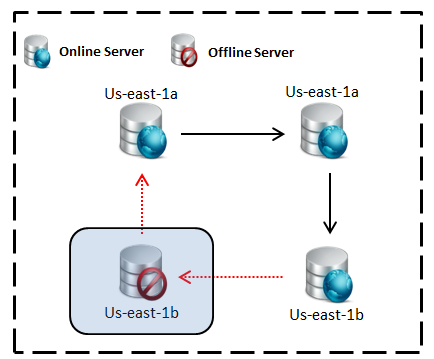
\includegraphics[scale=0.8]{Images/figure4.PNG}
\caption{\textbf{Automated Fail Stop Fault Detection:} In case of a server
failure the ring topology is broken and two neighbor servers (master and slave)
are affected. We detect this failure dynamically.} \label{fig:failuredetection}
\end{figure} It can be easily seen from \textbf{Figure
}~\ref{fig:connectreplication} that, if any one of the node fails, the ring will
be broken (\textbf{Figure }~\ref{fig:failuredetection}) and a partition between
instances will arise, which in turn will affect two of our goals, namely
consistency and availability. To address this, first we define the granularity
of failure we adopted. Failure can happen in one of three ways, those are (1)
the \emph{EC2} instance itself can go down, (2) the  \emph{Apache} web server
instance can fail or (3) the \emph{MySQL} can fail. Our policy is to take out
the failed instance from the cluster entirely if any of the above situations
occurs and thus eliminating the possibility of the failed instance being used by
any client. We do this in a two step process. First a robust failure detection,
followed by recovery. Both of these steps are automated and require zero human
intervention. \\ For failure detection we implemented a \emph{Gossip} type
protocol where each instance in the chain keeps track of its \emph{master}
instance. It collects two types of heartbeats, it periodically probes the
\emph{MySQL} service that covers the third failure scenario and secondly it also
probes the web server installed on the \emph{EC2} instance which detects the
first two failure scenarios. As mentioned earlier in this report, failure
detection and recovery are done by custom \emph{shell scripts}. Every instance
runs a failure detection script that monitors these heartbeats. In case of any
missing heartbeat, each instance dynamically repositions (recovery) itself to
the proper location and completing the chain (\textbf{Figure
}~\ref{fig:failurerecovery}). It is worth mentioning that, this recovery takes
less than a couple of seconds without interrupting any availability and raising
any inconsistent situation. This failure recovery module is also written in
shell script, which knows the address of all other instances and their
positions. Namely, each instance can go back ward and select a different master
when the original master has failed.  On the failed server, the same script
detaches the entire instance from the cluster in case of a missing \emph{MySQL}
heartbeat. The other two failure cases (web server and the \emph{EC2} instance
itself) are handled by the load balancer (see \textbf{Section} \ref{lb.a.t} ).
\begin{figure}[H]
\centering 
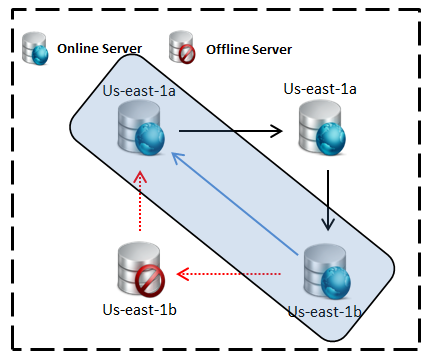
\includegraphics[scale=0.8]{Images/figure5.PNG}
\caption{\textbf{Automated Fail Stop Fault Recovery:} In case of a server
failure the ring topology is broken and two neighbor servers (master and slave)
are affected. The recovery script simply bridges the newly created gap between
these two endpoints.} 
\label{fig:failurerecovery} 
\end{figure} 
At this point we would like highlight few significant gains achieved from this simple failure
detection and recover model - 
\begin{itemize} 
\item Failure detection and recovery does not depend on the failed node(s) 
\item Any node can fail without affecting availability and consistency 
\item Failure detection and recovery processes are automated and fast 
\item As long as there is one functional instance alive, end-users will be able to access 
this service 
\item The entire process is absolutely transparent to the end-users 
\end{itemize} 
Once the original server is active and functional again, it will re-attach it self to the
appropriate \emph{master} (more on this in \textbf{Section }\ref{scalability} ),
and its heartbeat will be detected by the original \emph{slave} and that will
trigger the \emph{slave} to re-attach itself to the \emph{master} restoring the
topology to its ideal state. Once the restoration completes, the recently
recovered server starts getting all the missing updates from its \emph{master}
(assuming \emph{master} has not failed by then) and synchronizes the log
position. 

\subsection{Scalability}
\label{scalability} 
Once we designed the dynamic fault detection and recovery, we saw
that it inherently supports scalability with minimum effort. The scenario is
depicted in \textbf{Figure }~\ref{fig:scalability}. When a new server is brought
up online, the gliding in process showed in \textbf{Figure
}~\ref{fig:scalability} is exactly same when a failed server comes back on line
and relocate it self to the appropriate position in the ring. Therefore the
system can support addition of arbitrary number of servers with minimum
intervention except the following two. The new server will need a complete list
of available server's IP addresses and location information. As of now this list
will have to be manually embedded inside the new server's recovery script and we
consider this as a bootstrap requirement. The second important requirement is
that, the new server must have the right permission to access the existing
instances.  
\begin{figure}[H] 
\centering
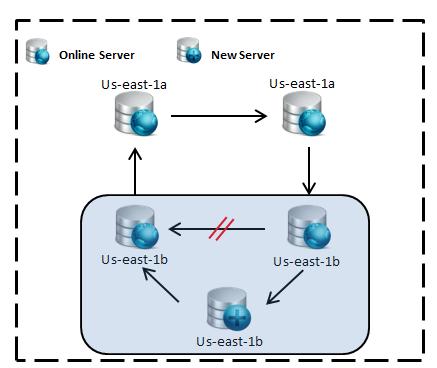
\includegraphics[scale=0.8]{Images/figure3.PNG} 
\caption{\textbf{Scalability:}
When a new server is added to the cluster, the bootstrap script (a.k.a recovery
script) automatically finds a suitable location for the new server to glide in.
We try to keep the servers from the same zone in close proximity. The bootstrap
script then automatically reconfigures the cluster to complete the ring topology
} 
\label{fig:scalability} 
\end{figure}

\subsection{Load balancing, Availability and Transparency}
\label{lb.a.t} We have
used amazon's default load balancing service provided as part of the \emph{EC2}
services, which is also an \emph{EC2} instance with minimum re-configuration to
implement our design. We refer to \textbf{Figure }~\ref{fig:workflow} to point
out the position of the load balancer in the overall layout. The load balancer
considers the system load in individual instance, its geographic location (in
\emph{EC2} terms) and the client's geographical location to forward a specific
request to a specific instance in the cluster. Besides, it abstracts out the
entire back-end and makes it absolutely transparent to the end-user. It also
maintains the membership of each instance in the cluster. Every transaction
aimed for the cluster internally or from client goes through the Load Balancer.
For example, as we mentioned in \textbf{Section }~\ref{fault} that we isolate an
instance from the end-user in the face of any type of failure. We achieve this
by manipulating the load balancer's configuration. Apart from our own monitoring
module, the load balancer constantly monitors the concerned ports (3306, 80 and
22) and excludes an instance if it fails to receive a heartbeat from any of
these ports, this makes the faulty instance unreachable from any client or even
from within the cluster (unless accessed using explicit IP address). In addition
to the load balancer we have an external domain name service that adds another
layer of abstraction to the design and can be configured to point to a different
cluster during system maintenance or catastrophic failure. However, updates in
DNS records propagates asynchronously through the Internet, and hence it may
take up to 6 hours (based on our experience) for the new information to be
propagated all the root DNS servers.

\section{Evaluation Of the Design and Results} We have conducted a number of
tests to evaluate our system's performance and desired features like consistency,
replication strength, scalability, load distribution and capacity in terms of
concurrent connections and queries. We only included three replicas in the chain
purposely due to the limitation imposed by \emph{EC2} \cite{freetier} on I/O and
data transfer. During this course we have written \emph{cronjobs}, several \emph{shell} and
\emph{MySQL} scripts to automate load generation, simulation and data
collection. The load configuration was different for the different tests. We
wrote a \emph{shell} script that uses \emph{mysqlslap} \cite{mysqlslap}, a tool
that comes with the \emph{MySQL} release to generate concurrent synthetic queries on
specified hosts with custom specification and schema. All the data presented in
the following subsections are real time and collected from the live system under
controlled environment.  
\subsection{Performance Improvement and Scalability} 
In this section we first present the limitation of a single \emph{MySQL} instance
in terms of concurrent writes it can accept and serve under a specific hardware
and system configuration. We then present the improvement achieved by replacing
a single instance with a cluster of three instances. For this part of the
simulation we varied the number of concurrent clients from 50 to 350, each
submitting a single query 100 times. And then we plot average, minimum and
maximum query completion time for each test set, however considering no abnormal skew, the average is considered
as it adequately reflects a reasonable negotiation of the both
measures. In the first part of the test we submitted the aforementioned workload
to a single \emph{MySQL} instance and collect these metrics. We spawned a fresh
instance for this purpose and directed the simulated load to that. In
\textbf{Figure }~\ref{fig:singlereplica} we can see the performance of a single
replica under varied workload. For exactly \emph{15000} queries the average
response time was about \emph{23.43} seconds.  
\begin{figure}[H] 
\centering
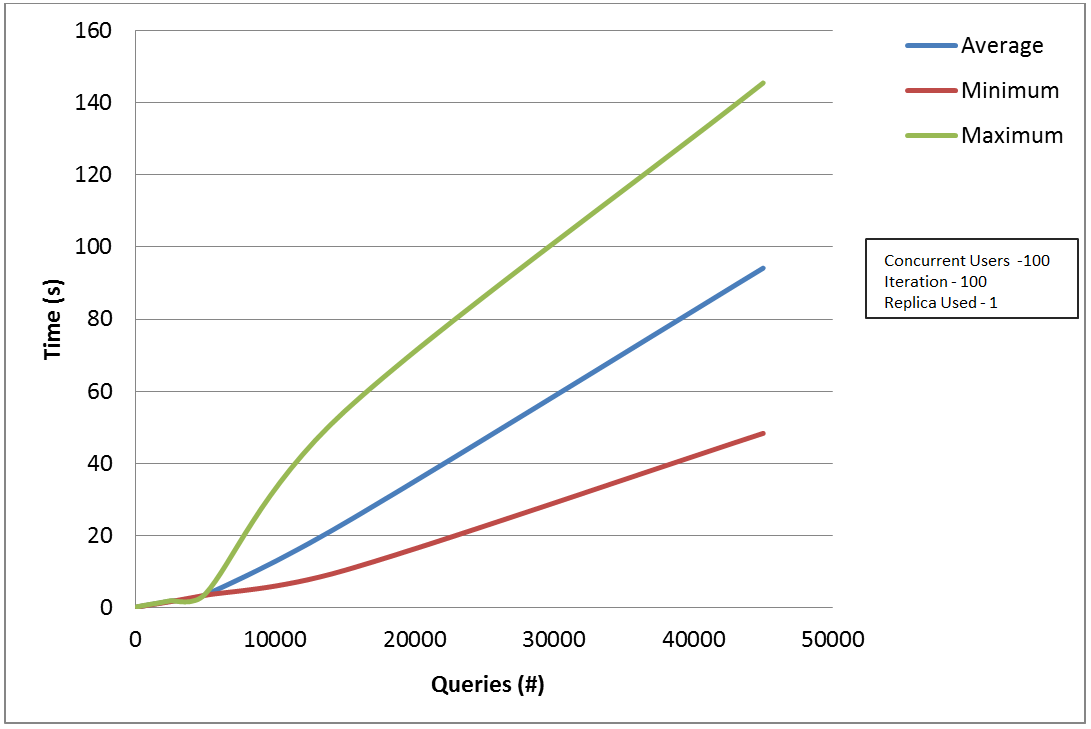
\includegraphics[scale=0.45]{Images/graph_singlereplica.PNG}
\caption{\textbf{Performance of a single MySQL instance:} This graph plots the
average, minimum and maximum query completion time against different test sets
involving varied number of concurrent queries. } \label{fig:singlereplica}
\end{figure} 
Next, we submit a similar workload to a cluster of three replicas
and report the results in \textbf{Figure }~\ref{fig:scaling}. A significant improvement 
in performance in terms of latency to serve each query is observed.
For exactly \emph{35000} queries the average response time was about \emph{2.6}
seconds. This indeed is a non-trivial improvement.  
\begin{figure}[H] 
\centering
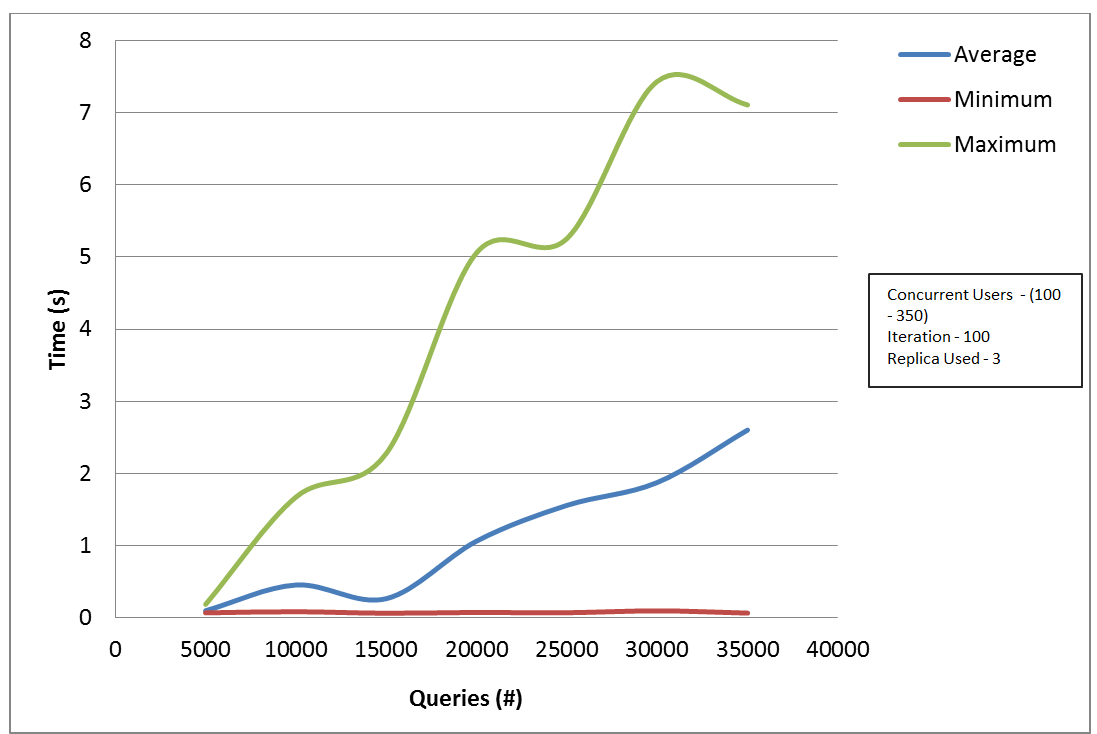
\includegraphics[scale=0.45]{Images/graph_scaling.PNG}
\caption{\textbf{Performance of a cluster of MySQL instances:} This graph plots
the same metrics for a similar workload against total number of queries
submitted to a cluster of three \emph{MySQL} instances. } 
\label{fig:scaling}
\end{figure} 
\subsection{Query Distribution \& Replica Performance} Next we
consider the performance of the load balancer. In other words we wanted to see
how well the system distributes requests under extreme work loads. For this we
simulated a \emph{350} concurrent clients from three \emph{EC2} instances, each
submitting \emph{100} queries to the cluster. \textbf{Figure
}~\ref{fig:lb_conns}, ~\ref{fig:lb_queries},~\ref{fig:lb_bytes_sent} and
~\ref{fig:lb_bytes_recv} depict the live scenarios in the three \emph{MySQL}
instances under this load. The first two show the number of concurrent queries
and connections while the other two present a measurement of incoming and
outgoing traffic. In all the four cases, the queries were distributed almost
evenly across the three servers, however \emph{server3} served more number of queries
as we tweaked the number of incoming connections in server 3 to allow more. In
addition to that, we wanted to see the reaction in the cluster in the face of a
failure. For that purpose, at approximately 130th second during simulation we
took down \emph{server1} and we can see that the remaining load was shared across the
remaining two servers almost instantly.  
 \begin{multicols}{2}
\begin{figure}[H] 
\centering
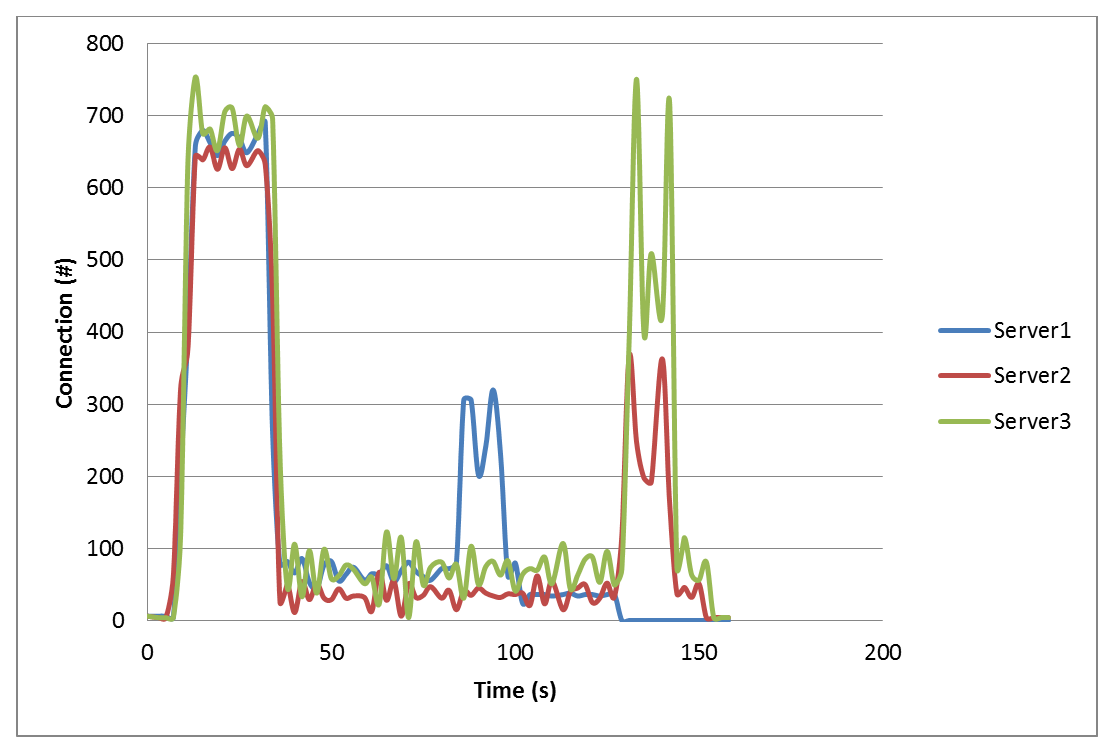
\includegraphics[scale=0.3]{Images/graph_lb_conns.PNG}
\caption{\textbf{Connection Distribution}  } 
\label{fig:lb_conns} 
\end{figure}

\begin{figure}[H] 
\centering
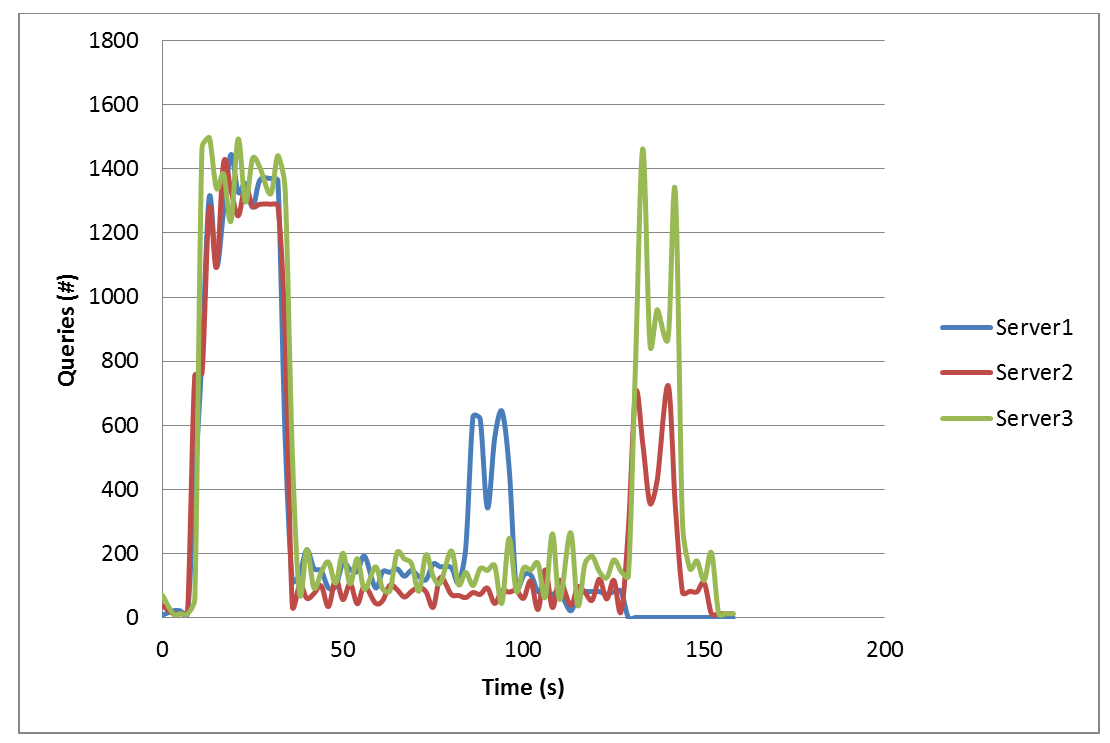
\includegraphics[scale=0.3]{Images/graph_lb_queries.PNG}
\caption{\textbf{Number of Queries Served by Each Instance} }
\label{fig:lb_queries} 
\end{figure} 
\end{multicols}

\begin{multicols}{2} 
\begin{figure}[H] 
\centering
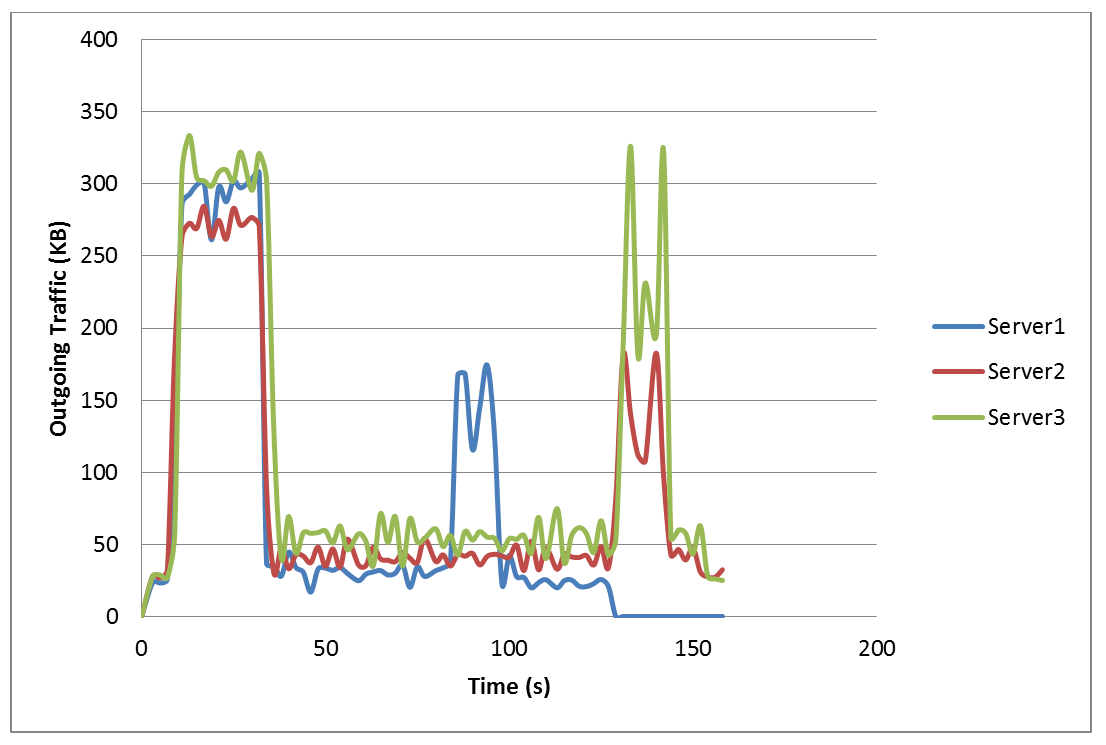
\includegraphics[scale=0.3]{Images/graph_bytes_sent.PNG}
\caption{\textbf{Outgoing Traffic} } 
\label{fig:lb_bytes_sent} 
\end{figure}

\begin{figure}[H] 
\centering
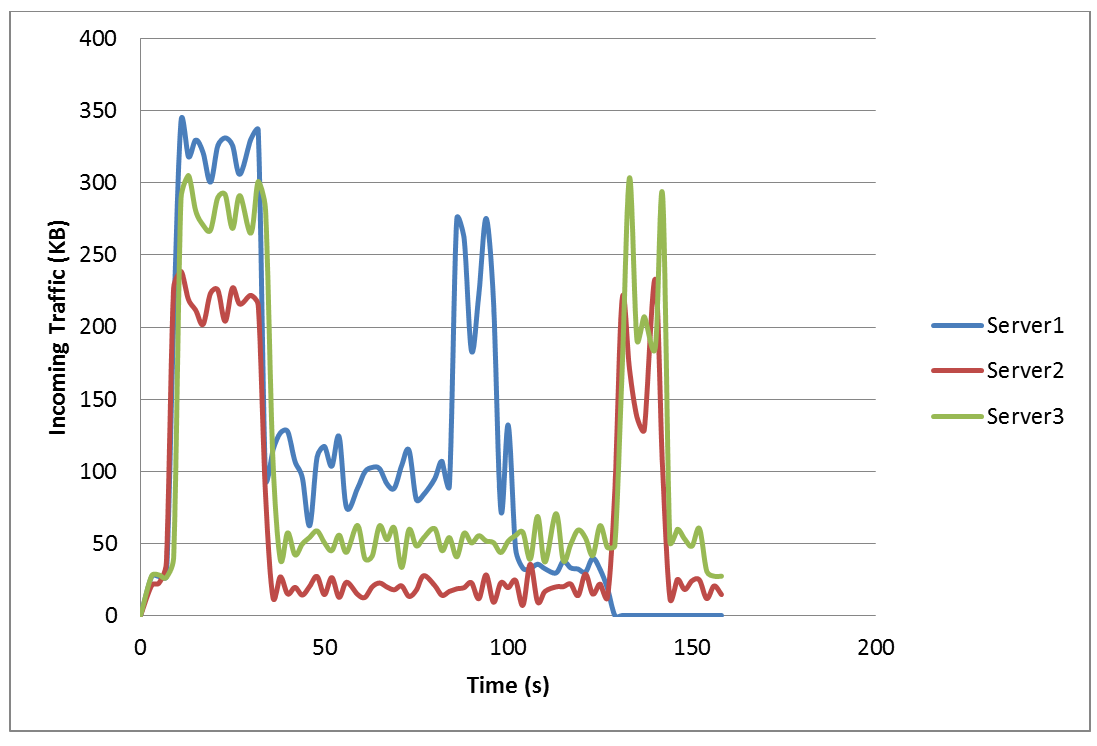
\includegraphics[scale=0.3]{Images/graph_bytes_recv.PNG}
\caption{\textbf{Incoming Traffic} } 
\label{fig:lb_bytes_recv} 
\end{figure}
\end{multicols} 

\subsection{Eventually Consistent Replication} To evaluate the
consistency strength of the system, we simply calculated the hash of each
\emph{MySQL} instance and compared with others in real time under extreme
load, distributed among the members in the cluster. This can be seen as taking a
snapshot of all the tables and performing a comparison of those snapshots. To do
this we used a third party tool \emph{mk-table-checksum} \cite{mk-table}, a part
of \emph{maatkit} \cite{maatkit} package. This program simply helps one to
calculate checksum of specific database in a specified host. The load
configuration for this test was, \emph{250} simulated concurrent clients from
each \emph{EC2} instance submitting a single query \emph{100} times. And we
simultaneously generated similar load from all the the \emph{EC2} instances. So
the total number of concurrent queries submitted to three \emph{MySQL} cluster
was \emph{(250 x 100 x 1) x 3} = 75000. A separate script on a remote machine
calculated the checksum of these three replicas every \emph{2} seconds while the
queries were being served by the cluster and reported the checksums. In
\textbf{Figure }~\ref{fig:consistency}, we report the outcome of this test. We
can see from this graph that, the three checksums are not far away from each
other and most of the time they are equal. And eventually after a certain period
they reach to a consistent state. This lag period varies and depends on the
transmission delay between any two instances, and in our case it was less 10
seconds under significant work load. This proves our claim of eventual
consistency provided by the cluster.  

\begin{figure}[H] 
\centering
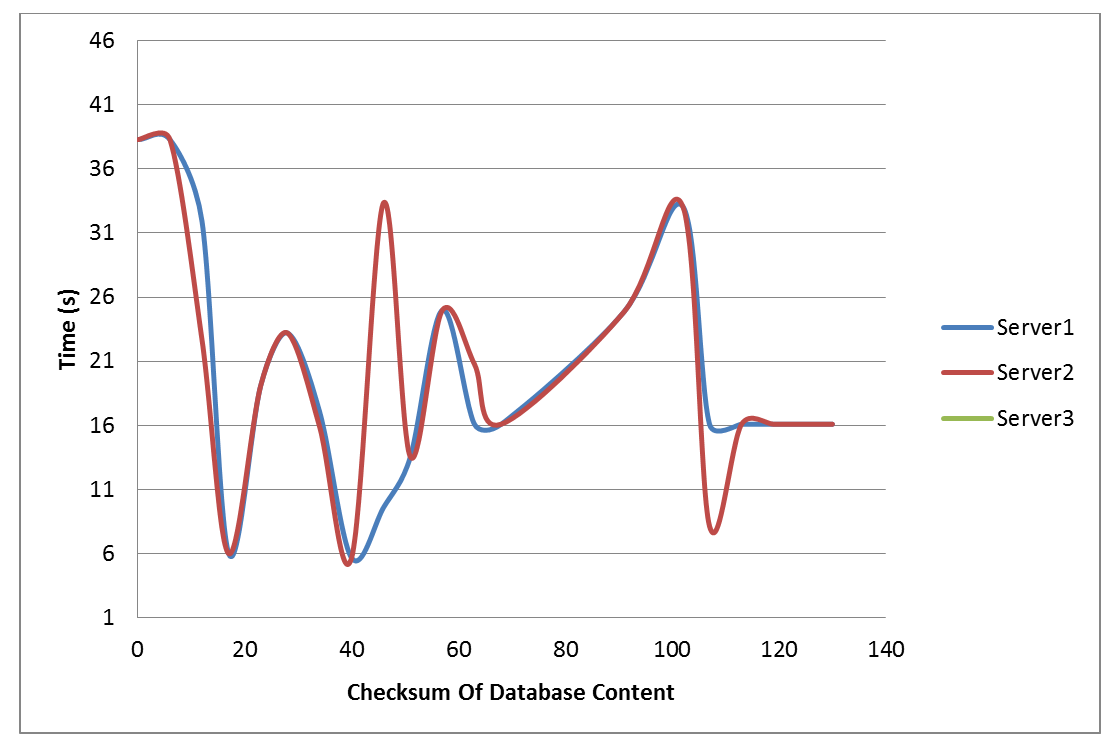
\includegraphics[scale=0.35]{Images/graph_consistency.PNG}
\caption{\textbf{Verifying Eventual Consistency through MySQL Instance Checksums: This 
graph plots the checksum of MySQL instances versus time.}
}
\label{fig:consistency} 
\end{figure} 
\subsection{Overloading the Web Server and Evaluation of Stress Test} In order to 
evaluate loading balancing and availability, Apache's JMeter was utilized. JMeter 
is a well tested tool to load test functional behavior and measure 
performance\cite{apache}. Load was tested under the original setup of 4 instances 
with 10, 100 and 500 users. The 3
experiments were repeated for set of 3, 2 and 1 instance. A linear increase in
number of users versus latency was observed. The latency also linearly decreased
with an increase in number of instances \textbf{Figure} ~\ref{fig:median_latency}. Min
latency(ms) was fairly consistent except in the case of 4 instances simulated
with 100 users \textbf{Figure} ~\ref{fig:min_latency}. An interesting trend was observed for max
latency. We expected max latency to increase with number of users and decrease
with increase in number of instances. However, the max latency increased with an
increase in number of instances. This behavior may be due to outliers. However,
since we observe an overall increase in latency with increase in instances(as
suggested by median and average date), we are confident that availability
decreases latency.  

\begin{multicols}{2}
\begin{figure}[H] 
\centering
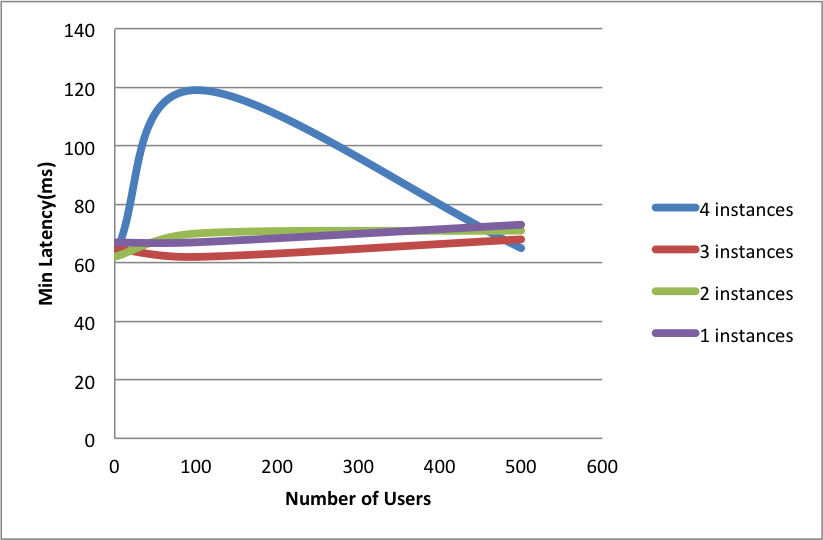
\includegraphics[scale=0.6]{Images/min_latency.PNG} 
\caption{\textbf{Min Latency} This graph plots number of simulated users versus min latency(ms). 
Min latency is independent of number of instances or users} 
\label{fig:min_latency}
\end{figure} 

\begin{figure}[H] 
\centering
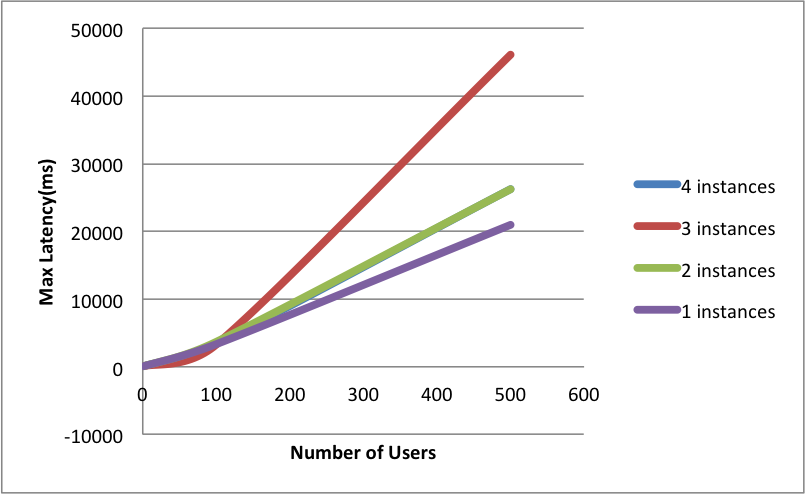
\includegraphics[scale=0.64]{Images/max_latency.PNG} \caption{\textbf{Max
latency} This graph plots number of simulated users verus max latency(ms). Min latency 
increases with an in number of instances and users } 
\label{fig:max_latency} 
\end{figure} 
\end{multicols}

\begin{figure}[H] 
\centering
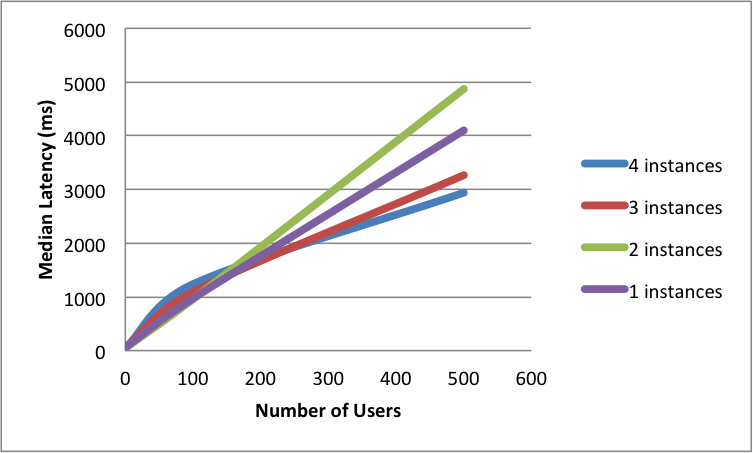
\includegraphics[scale=0.75]{Images/median_latency.PNG} 
\caption{\textbf{Median
latency} This graph plots number of users versus median latency (ms). Median latency 
increases with increase in number of users and decrease in number of available instances} 
\label{fig:median_latency} 
\end{figure}

\section{Source Control} 
Apart from the scripts that we wrote for implementing the distributed environment, 
we wrote a couple of simple scripts for source control and updating source files in all the three
instances. We used \emph{Github} \cite{github} to store our source codes and the
\emph{cronjobs} inside each \emph{EC2} instance periodically checks the {Github}
repository and updates the necessary source files in the web server. Of course
this can also be manually triggered if necessary.

\section{Limitation \& Future Work}
In the previous sections we claimed and showed that the all the replicas in the
\emph{MySQL} cluster reach to a consistent state eventually. The update
propagation happens eventually because each query submitted by a client is only
written to one replica before returning to the client. The propagation is
asynchronous and depends on latency between two replicas. However, a more
complex algorithm can be implemented and used on this current configuration
which will propagate the update in a semi-synchronous or even synchronous
manner. The idea is to \emph{try} to perform the submitted query on $n$ ($n >
1$) replicas before getting back to the client. For this project we did not
explore this option as the notion of eventual consistent replicas is strong
enough for our client application (distributed message system) and the
complexity of the algorithm required for this semi-synchronous update mechanism
is dwarfed by the replication performance of the existing simple asynchronous
design. Secondly, we have written bash scripts to automate failure detection,
recovery and to make the system scalable. However, the topology information
(e.g. location and IP addresses of the instances) are hard coded as of now. We
originally planned to come up with a dynamic configuration file that these
scripts can read from and write to and a tool to manage these configuration
files from a single instance, but due to time constraint we could not reach that
point. Nevertheless, the scripts work just fine. We introduced the functionality
and position of the system\rq{}s \emph{load balancer} in \textbf{Section }
\ref{lb.a.t}. This \emph{load balancer} is indeed a single point of failure and
currently we do not have any shadow instance to substitute the failed \emph{load
balancer}. But as the \emph{load balancer} in our design does very specific job
it is very unlikely to be failed due to higher number of requests. In any case,
coming up with a secondary \emph{load balancer} should be pretty straight
forward. 

\section{Conclusion}
This paper describes the design, implementation and performance evaluation of a
communication tool built upon distributed system principles. We show that
replication increases data availability and improves performance. Further, we
show that our application is efficiently able to load balance and execute
various \emph{MySQL} queries in parallel. Time permitting, we would have further liked
to expand our design and implement a shadow or backup server for the load
balancer as well as further automate process of server configuration.

\begin{thebibliography}{99} 
\bibitem{lamport} Lamport, L., {\it LaTeX : A
Documentation Preparation System User's Guide and Reference Manual},
Addison-Wesley Pub Co., 2nd edition, August 1994.  
\bibitem{IRC} J. Oikarinen and D. Reed, “Internet Relay Chat Protocol RFC 1495,” 1993.  
\bibitem{apache} \url{http://www.apache.org} 
\bibitem{ec2}  \url{http://aws.amazon.com/ec2}
\bibitem{connect}  \url{http://connect.microwebpla.net} 
\bibitem{t1micro} \url{http://aws.amazon.com/ec2/instance-types}
\bibitem{freetier}\url{http://aws.amazon.com/ec2/pricing} 
\bibitem{mysql} \url{http://www.mysql.com} 
\bibitem{jquery} \url{http://www.mysql.com}
\bibitem{cname} \url{http://en.wikipedia.org/wiki/CNAME\_record}
\bibitem{mysql-replication} \url{http://dev.mysql.com/doc/refman/5.0/en/replication.html} 
\bibitem{mk-table} \url{http://www.maatkit.org/doc/mk-table-checksum.html} 
\bibitem{maatkit} \url{http://www.maatkit.org} 
\bibitem{mysqlslap} \url{http://dev.mysql.com/doc/refman/5.1/en/mysqlslap.html} 
\bibitem{github} \url{http://github.com} 
\end{thebibliography} 

\end{document}
